\chapter{Marco Metodológico}
\markboth{Marco Metodológico}{Marco Metodológico}

\section{Metodologia Fundacional para la Ciencia de Datos}
    \lhead[\thepage]{\thesection Metodologia Fundacional para la Ciencia de Datos}

    Según \cite{foundationalmet} en el ámbito de la ciencia de datos, una metodología es una estrategia general que guía los procesos y actividades en un dominio dado. La metodología no depende de herramientas o tecnologías en particular, ni es un conjunto de técnicas o récipes. Mas bien, una metodología provee al científico de datos con un marco de trabajo de como proceder con cualquier método, procesos y heurísticas que sean usadas para obtener respuestas o resultados.


    Resolver problemas y responder preguntas a través de análisis de datos es una practica estandarizada en ciencia de datos, como meta principal del área esta el obtener información del proceso de análisis, que luego es utilizada por las organizaciones para tomar alguna acción requerida por la misma.\cite{foundationalmet}

    La Metodologia Fundacional para la Ciencia de Datos propuesta en \cite{foundationalmet} busca establecer un marco de trabajo que cumpla con la definición de metodología del autor y provea una guia de estrategias independiente de la tecnología, volumen de los datos o abordaje.


    \begin{figure}[htpb]
        \centering
        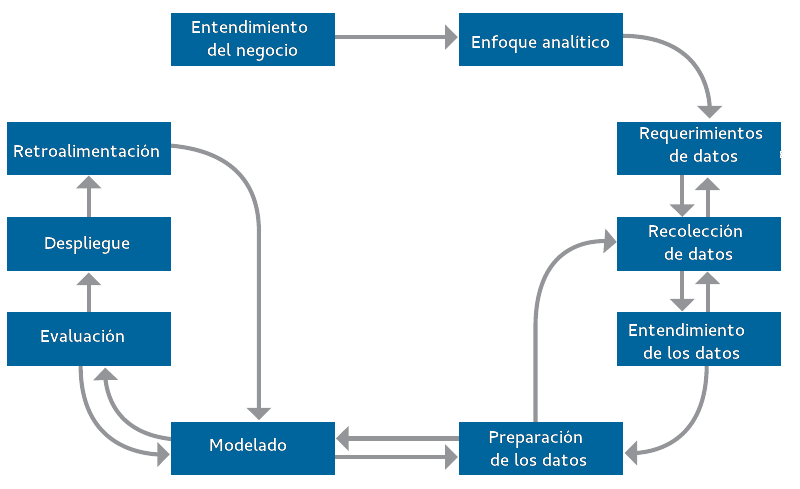
\includegraphics[width=0.85\textwidth]{Figuras/foundational_met_image.png}
        \caption{Metodologia Fundacional para la Ciencia de Datos}
        \label{fig:foundmetfig}
    \end{figure}

    En la Figura \ref{fig:foundmetfig} se muestra la metodología de 10 fases propuesta en \cite{foundationalmet}. Este marco de trabajo posee algunas similitudes con metodologías reconocidas para minería de datos, pero enfatiza varias de las nuevas practicas en ciencia de datos como el uso de grandes volúmenes de datos, la incorporación de análisis de texto en modelos predictivos y la automatización de algunos procesos.

    \subsection{La 10 fases de la Metodologia Fundacional para la Ciencia de Datos}
    \begin{enumerate}
        \item Entendimiento del negocio (\emph{Business understanding}): Sin importar el tamaño o alcance de un proyecto, este debe comenzar por la comprensión del negocio, de dicho entendimiento dependerá en gran medida el éxito de la solución al problema. Es vital para los representantes del negocio que la solución analítica sea fundamental en esta etapa mediante la definición del problema, los objetivos del proyecto y los requerimientos de la solución.
        \item Enfoque analítico (\emph{Analytic approach}): Una ves definido el problema el científico de datos estable el enfoque analítico. Para ello el problema es expresado en técnicas de \emph{machine learning} para que  el científico de datos logre identificar cuáles son las técnicas que mejor se adaptan para conseguir los resultados deseados.
        \item Requerimientos de datos (\emph{Data requirements}): La elección del enfoque analítico determina los requerimientos de datos. Los métodos analíticos a usar requieren contenido, formato y representaciones particulares de los datos.
        \item Recolección de datos (\emph{Data collection}): Las fuentes de datos (estructurados, no estructurados, semi-estructurado) relevantes para el dominio del problema son identificadas y agrupadas por el científico de datos. En caso de encontrar brechas en la recolección de datos, podría ser necesario revisar los requerimientos de datos y recolectar más datos.
        \item Entendimiento de los datos (\emph{Data understanding}): El científico de datos debe entender el contenido de los datos, evaluar su calidad y descubrir características de interés para ello se puede apoyar en técnicas de visualización y estadísticas descriptivas.
        \item Preparación de los datos (\emph{Data preparation}): Actividades que incluyen la limpieza de datos, combinación de múltiples fuentes y transformación de datos en variables más prácticas, que preparan los datos para ser usados en la etapa de  modelado.
        \item Modelado (\emph{Modeling}): A partir de una versión inicial del conjunto de datos preparado, el científico de datos utiliza conjuntos de entrenamiento (datos históricos de los cuales los resultados son conocidos), para desarrollar modelos predictivos o descriptivos utilizando el enfoque analítico anteriormente descrito. Esta etapa es altamente iterativa.
        \item Evaluación (\emph{Evaluation}): La evaluación de la calidad del modelo implica verificar si este
        dirige el problema de forma completa y apropiada. Esto requiere que el científico de datos aplique distintos diagnósticos y medidas computadas utilizando el conjunto de entrenamiento y el modelo predictivo.
        \item Despliegue (\emph{Deployment}): Con un modelo satisfactorio, aprobado por los representantes del negocio, se procede al despliega dentro del ambiente de producción u otro ambiente de prueba equiparable, para poder obtener una evaluación de su rendimiento.
        \item Retroalimentación (\emph{Feedback}): Recolectando los resultados obtenidos luego de la implementación de la fase de despliegue, la organización obtiene datos sobre el rendimiento del modelo y observa como el mismo afecta el ambiente de producción. Analizar dicha dicha información permite a los científicos de datos refinar el modelo, incrementar su precisión y con esto su utilidad.
    \end{enumerate}

\section{Modelo CRISP-DM}
\lhead[\thepage]{\thesection Modelo CRISP-DM}

CRISP-DM concebido en 1996, es el acrónimo en ingles de \textit{Cross Industry Standard Process for Data Mining}. Fue creado con la meta de ser una metodología estándar, neutral a industria, herramienta o aplicación.\cite{chapman2000crisp}


En \cite{chapman2000crisp} esta metodología es descrita en términos de un modelo de procesos jerárquicos, consiste de cuatro niveles tal como se muestran en la Figura \ref{fig:crispniveles}.

\begin{figure}[H]
    \centering
    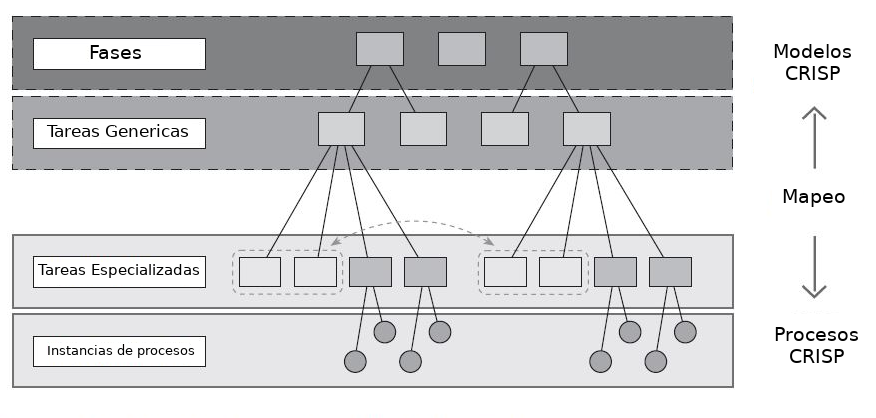
\includegraphics[width=0.7\textwidth]{Figuras/niveles_crisp.png}
    \caption{Los 4 niveles de la metodología CRISP-DM}
     \source{http://crisp-dm.eu/wp-content/uploads/2013/03/Four-Level-Breakdown-of-the-CRISP-DM-Methodology.jpg}
    \label{fig:crispniveles}
\end{figure} 

El primer nivel consta de fases, cada una de estas consiste en varias tareas genéricas (\emph{Generic Taks}), dichas tareas intentan ser lo suficientemente generales como para cubrir todas las posibles situaciones de minería de datos. Buscan ser completas, esto es, cubrir tanto los procesos como aplicaciones de la minería de datos. Estables, el modelo debe ser valido para nuevos desarrollos como nuevas técnicas de modelado.\cite{chapman2000crisp}

En el tercer nivel, el nivel de las tareas especializadas(\emph{Specialized Task}) se describen como deben llevarse acabo, bajo ciertas situaciones, las acciones en el segundo nivel. En el cuarto nivel, la instancias de procesos (\emph{Process Instances}), es un registro de acciones, decisiones y resultados de un abordaje real de minería de datos. Una instancia de proyecto es organizada de acuerdo a la tarea definida en los niveles superiores, pero representa lo que realmente pasa en un - particular, que lo que pasa en general.\cite{chapman2000crisp}


\begin{figure}[H]
    \centering
    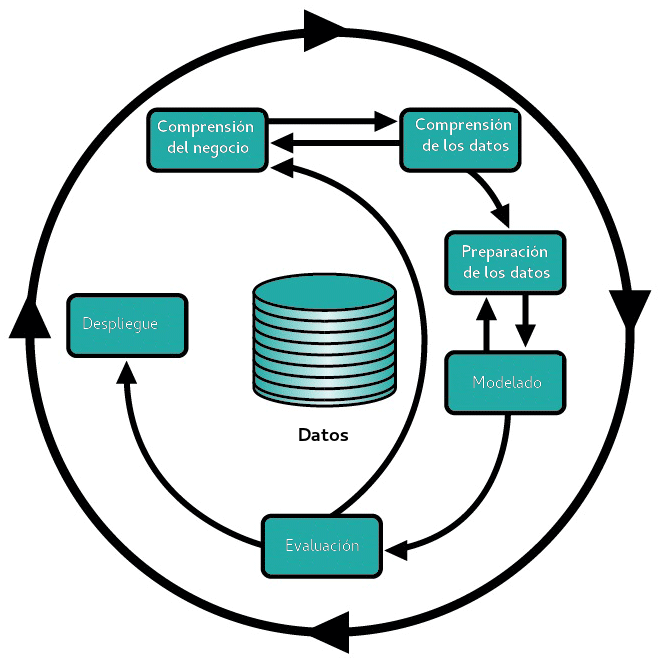
\includegraphics[width=0.85\textwidth]{Figuras/crip_fases.png}
    \caption{Las 6 fases del proceso de minería de datos}
     \source{http://crisp-dm.eu/wp-content/uploads/2013/07/newcrispdiagram.gif}
    \label{fig:crispfases}
\end{figure} 


La Figura \ref{fig:crispfases} muestra las fases de un proceso de minería de datos según el modelo de referencia de CRISP-DM. La secuencia entre las fases es flexible. Depende del resultado obtenido en cada fase cual fase sera la siguiente o que tarea particular de una fase sera llevada a cabo. Las flechas indican las dependencias mas importantes y frecuentes entre fases. El circulo exterior en la Figura \ref{fig:crispfases} indica la naturaleza ciclica del proceso de minería de datos.\cite{chapman2000crisp}

Siguiendo lo descrito en \cite{chapman2000crisp} cada una de las fases y sus principales tareas son :
\begin{enumerate}
   
 \item Comprensión del negocio (Objetivos y requerimientos desde una perspectiva no técnica)
    \begin{enumerate}
    \item Establecimiento de los objetivos del negocio (Contexto inicial, objetivos, criterios
    de éxito).
    \item Evaluación de la situación (Inventario de recursos, requerimientos, supuestos,
    terminologías propias del negocio).
    \item Establecimiento de los objetivos de la minería de datos (objetivos y criterios de
    éxito).
    \item Generación del plan del proyecto (plan, herramientas, equipo y técnicas).
    \end{enumerate}

 \item  Comprensión de los datos (Familiarizarse con los datos teniendo presente los objetivos
del negocio)
    \begin{enumerate}
    \item Recopilación inicial de datos.
    \item Descripción de los datos.
    \item Exploración de los datos.
    \item Verificación de calidad de datos.
    \end{enumerate}

 \item  Preparación de los datos (Obtener la vista minable o \textit{dataset})
    \begin{enumerate}
    \item Selección de los datos.
    \item Limpieza de datos.
    \item Construcción de datos.
    \item Integración de datos.
    \item Formateo de datos.
    \end{enumerate}

 \item  Modelado (Aplicar las técnicas de minería de datos a las vistas minables)
    \begin{enumerate}
    \item Selección de la técnica de modelado.
    \item Diseño de la evaluación.
    \item Construcción del modelo.
    \item Evaluación del modelo.
    \end{enumerate}

 \item Evaluación (De los modelos de las fases anteriores para determinar si son útiles a las
necesidades del negocio)
    \begin{enumerate}
        \item Evaluación de resultados.
        \item Revisar el proceso.
        \item Establecimiento de los siguientes pasos o acciones.
    \end{enumerate}

 \item  Despliegue (Explotar utilidad de los modelos, integrándolos en las tareas de toma de
decisiones de la organización)
    \begin{enumerate}
       \item Planificación de despliegue.
    \item Planificación de la monitorización y del mantenimiento.
    \item Generación de informe final.
    \item Revisión del proyecto.
    \end{enumerate}


\end{enumerate}
